%%%%%%%%%%%%%%%%%%%%%%%%%%%%%%%%%%%%%%%%%%%%%%%%%%%%%%%%%%%%%%%%%
%%%  Capstone Project Template that tries to save a few trees %%%
%%%  Edwin Blake 22 Aug 2013                                                   %%%
%%%		1 Aug 2014 (revised)                                      %%% 
%%%  see also                                                                             %%%
%%% http://ravirao.wordpress.com/2005/11/19/latex-tips-to-meet-publication-page-limits/  
%%%%%%%%%%%%%%%%%%%%%%%%%%%%%%%%%%%%%%%%%%%%%%%%%%%%%%%%%%%%%%%%%

\documentclass[11pt,a4paper]{article}
\usepackage{times}
\usepackage{fancyhdr}           % Allows better control over headers and footers
%\usepackage{layout}            % use with \layout to see the page layout for
%debugging purposes.
\usepackage[margin=2.5cm]{geometry}  %   set the margins using the
                                %   geometry package (which is much
                                %   the easiest way of doing this).
\usepackage[pdftex]{graphicx}   %   Pictures (means you have to
                                %   produce pdf output via pdflatex)
\usepackage[small,compact]{titlesec}   % Try to reduce the white space
                                % latex loves so much
\titlelabel{\thetitle. \quad}   % Reduce space around section heads
                                % and add a full stop after the number
\pagestyle{fancy}               % Invoke fancy headers

\renewcommand{\abstractname}{\vskip -5mm}  %  Change name of Abstract
                                %  to nothing and loose some of the
                                %  excessive white space


\begin{document}

\title{Cheaters Plagiarism Detection Report} \date{}
\author{Merishka Lalla\\joe@bloggs.com
\and Yaseen Hamdulay\\jane.doe@uct.ac.za
\and Jarred de Beer\\john.doe@uct.ac.za}

%%%  Set the headers via fancyhdr package
\lhead{Capstone Project Report}  % Short title for running head
\chead{}
\rhead{1st August, 2014}   %  Fixed running head of the date
\lfoot{}
\cfoot{\thepage}    %  add page number as centre footer.
\rfoot{}
\renewcommand{\headrulewidth}{0.0pt}   % Don't want horizontal line
                                % under header.

\maketitle
\thispagestyle{plain}  % First page is plain style headings and
                       % footers (ie just the page number as footer).

\section*{Abstract}
The purpose of this project is to identify cheating among Computer Science
students when submitting their assignments. It is estimated that
30\% of students will cheat in an assignment, often sharing the code in groups amongst themselves.
 Our goal is to detect such occurrences and display the results for lecturer administration. 
We began by building a prototype, basing the algorithm on the proprietary JMoss system, 
but using only Python. We found our implementation worked well but failed in that it detected single lines 
of common and insignificant code, also, the initial UI could not display the high number of results
being listed. After refactoring our solution was to perform String matching, generating 
signatures on the text and filtering them for multiple lines of
recurring code, further comparing it with as an abstract syntax tree for subtree pattern matching. 
To test the algorithm was run against 18658 python assignments, yielding the same 30\% mean
of students cheating and deviating on the confidence interval with each occurrence by just 0.5\%
as given by the JMoss system. In conclusion our solution performs alongside JMoss, yet differs in its UI by
grouping cheaters to recurring code blocks, a more convenient view to administer cheating.

\section{Introduction}
\label{s:introduction}

The purpose of this project is to detect cheating among Computer Science
assignment hand-ins. The detection system plugs in to the student submission process on
Vula and will extract the source files to generate signatures on the source code and match
it with existing signatures. A front end web UI was built to list the offending students and
provide administration functionality for the convening lecturer to take action when needed. The web UI
is accessed from an iframe within the Vula dashboard, accessible by convening lecturers.
In general a lecturer will use this facility to verify code diffs against
students' code which has been marked as cheated and assign them zero for the assignment.

In some cases an assignment will be used over consecutive years, largely unchanged, if at all.
We therefore need the ability to compare code against not just the current year of submission
but also previous years.

The programming languages used for assignments differ from year to year, differing in some cases
even within the same year. It was therefore necessary to detect the appropriate programming language 
used with each submission. The Computer Science department makes extensive use of Python and Java for
assignments and so these are provided as plugins by default. The system has a plugin sub-system
which can be used to write parsers for additional languages, extending the scope of languages used
to detect cheating from within the department and allowing flexibility in terms of language support for
the future.

The software engineering methods used were traditional analysis followed by design and
implementation. An evolutionary prototype was constructed and presented to the stakeholders
for review, after which we analyzed the feedback and made use of Extreme programming to iterate over the product to get it into its
final state. Pair programming was used to ensure members were all on the same page and had
a shared working knowledge of the code and state of the project. This was advantageous especially
when refactoring code because during development small, technical issues would become
apparent. We were able to discuss such issues immediately, design and implement alternate
solutions, and modify existing methods or classes. The source code was checked out from
a git repository and the team members could then conveniently update their source code copies
after a peer programming session and work on the files individually, safely pushing detailed
commits with changes for other team members to remain up to date.

The core of the system, the algorithm detection, is based largely on the proprietary
JMoss system and was referenced while building the Winnowing algorithm as part of the
signature generation and matching. We were able to use the output from a provided database of
over 18000 python assignment files from the 1st year Computer Science course and compare
our implementation to the results given by JMoss on the same files. This was used also for
tweaking parameters to the system and gaining accuracy.

[TODO: insert reference, http://theory.stanford.edu/~aiken/publications/papers/sigmod03.pdf]

Your introduction provides the context for the project and should
contain the statement of the scope of the project (which may have
changed since you first wrote it). Someone reading your introduction
must have clear idea of what the system is intended for. If you think
there is something special about the kind of problem you tackled that
your reader needs to know up front then this is where you say it.

If you need any survey of other work (you probably don't) then put it
towards the end of the introduction and give suitable references. A
case where this is needed is if your project builds on someone else's
project or some published algorithm.

Discuss your approach to solving the problem. Please give a short
overview of the software engineering methods you used (e.g.,
traditional analysis followed by design and implementation -- typically
the case if you did an evolutionary prototype, or a more agile
approach where you had a cyclical development process). 

\section{Requirements Captured}

The next section deals with the analysis of your system. Cover the
functional, non-functional and usability requirements. This is where
you present your use case narratives and diagrams. 

Discuss the major analysis artefacts that you produced. We will expect
you to produce at least one overall description of the architecture
used in your system as a diagram, either here or below (see Section
\ref{s:design-overview}). You may also want to include an analysis
class hierarchy diagram.

\section{Design Overview}
\label{s:design-overview}

The next section is an overview of your design. The system design has
to be justified in terms of the expected behaviour of the final
product. 

If you produced a design class diagram put it here.

\begin{figure}[h!]
  \center{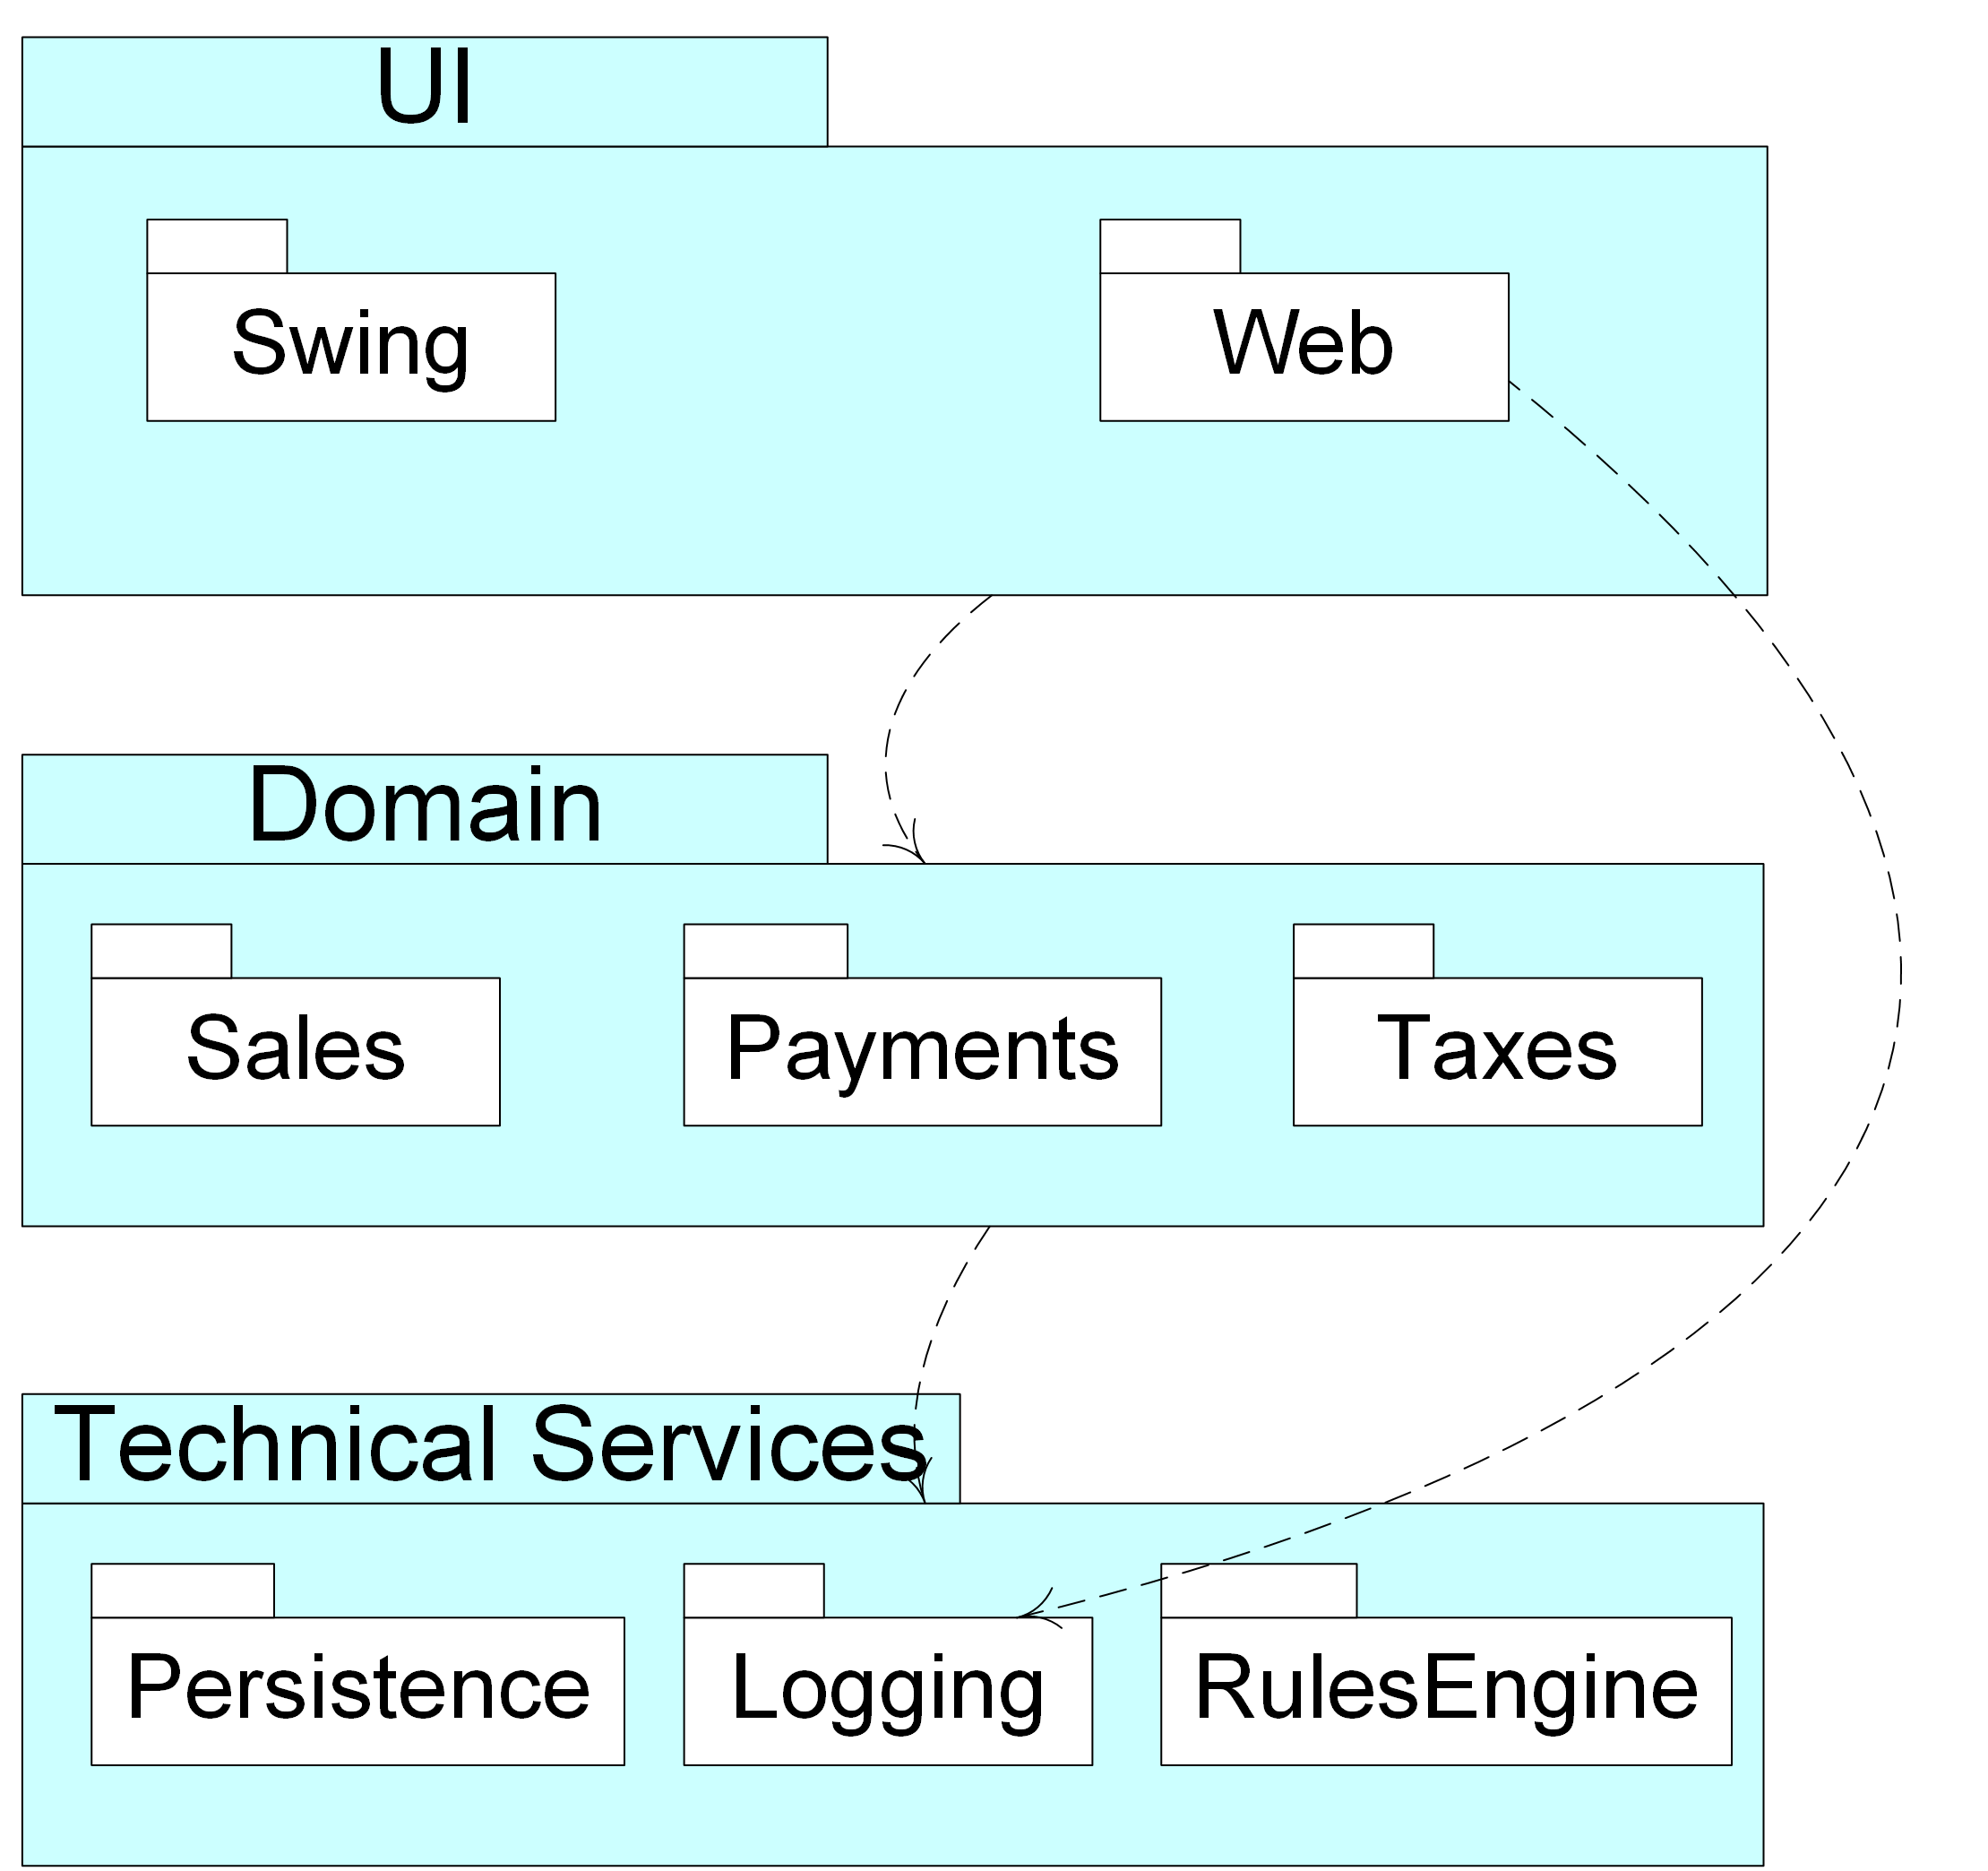
\includegraphics[scale=0.8]{architecture.png}}
  \caption{An architecture diagram. Caption to go below figure}
  \label{fig:architecture}
\end{figure}

You must present the overall architecture of the system together with
an architecture diagram. You may choose what kind of diagram best
suits your project but we would expect a layered architecture diagram
(see Figure \ref{fig:architecture}) unless there is a good reason for
some other kind of diagram. It need not be a formal UML diagram as
long as it conveys all the necessary information clearly.

You should then (in subsections) cover the algorithms and the data
organisation used and why they were considered the best. 

\section{Implementation}

Now we get to the details. 

\begin{itemize}
\item Describe your data structures and be sure to illustrate them
  with a diagram.

\item If your user interface was a key feature describe how that was
  implemented.

\item Discuss the function of the most significant methods in each
  class. This may well require flowcharts, or sequence diagrams, in
  some cases.

\item Any special relationship between the classes (e.g. friends) and
  why they exist.

\item A description of any special programming techniques or libraries
  used.
\end{itemize}

\section{Program Validation and Verification}
\label{ss:progr-valid-verif}

Tell us how you tested the system and why you believe it works.
Describe all the steps taken to validate the correctness of the
program.

If you had user tests then say what you did and what the results
were. Describe why these test data were chosen (what test conditions
the data was testing).  Table \ref{tab:tests} provides an example of
the sorts of results we are looking for. The full detail of the test
runs should be appended to the report.

\begin{table}[h!]
  \centering
\caption{A table of tests. A table caption goes above the table.}

  \begin{tabular}[t]{|p{5cm}|p{3cm}|p{3cm}|p{3cm}|} \hline \textbf{Data Set
    and reason for its choice} & \multicolumn{3}{c|}{\textbf{Test Cases}}\\
    \cline{2-4} & \emph{Normal Functioning} & \emph{Extreme boundary cases} &
    \emph{Invalid Data (program should not crash)} \\ \hline Preliminary test
    (see Appendix 3) & Passed & n/a & Fell over \\\hline &&&\\ \hline
    &&&\\ \hline
  \end{tabular}

\label{tab:tests}
\end{table}

Follow your table of results with a discussions of them highlighting
how useful and usable your system is for its intended purpose.

\section{Conclusion}
\label{ss:conclusion}

Your report must have a clear conclusion where you revisit the aims
set out in the beginning and discuss how well you met them. Did you
achieve the objective of creating a well-structured, modular, and
robust system?  Please summarize the design features and test results
that show this.

\begin{thebibliography}{9}

\bibitem[Kopka and Daly(2004)]{KopkaDaly}
Kopka, H. and Daly, P.W.  (2004) \textit{A Guide to \LaTeXe:
Document Preparation for Beginners and Advanced Users} (4th~edn).
Addison-Wesley.

\bibitem[Lamport(1994)]{Lamport}
Lamport L. (1994) \textit{\LaTeX: A Document Preparation System}
(2nd~edn). Addison-Wesley.

\bibitem[Mittelbach and Goossens(2004)]{Companion}
Mittelbach, F. and Goossens, M., (2004) \textit{The \LaTeX\
Companion} (2nd~edn). Addison-Wesley.

\end{thebibliography}
\end{document}
